\documentclass[10pt,a4paper]{article}
\usepackage[utf8]{inputenc}
\usepackage[french]{babel}
\usepackage[T1]{fontenc}
\usepackage{lmodern}
\usepackage{amsmath}
\usepackage{amsfonts}
\usepackage{amssymb}
\usepackage{graphicx}
\usepackage{subfigure}
\usepackage{subfig}
\usepackage{natbib}
\usepackage{layout}
\usepackage{wrapfig}
\usepackage{minitoc}
\usepackage{url}
%\usepackage{caption}
%\usepackage{subcaption}


\usepackage[top = 2.5 cm, bottom = 2.5 cm, left = 2.5 cm, right = 2.5 cm]{geometry}
\usepackage{listings}

\author{Philippe Verbist - Antoine Paris \\ \ \ \ 3521-13-00\ \ \ \ \ \ 3158-13-00}
\title{\textbf{Rapport du projet DJ'Oz}}
\date{Le 4 décembre 2014}
\begin{document}
\sloppy
\maketitle

\section{Structure du programme}
Comme il nous l'a été demandé, nous avons divisé notre programme en trois parties:
\begin{itemize}
	\item une fonction Interprete, qui prend une partition en paramètre et renvoie une liste d'échantillons;
	\item une fonction Mix, qui 1) prend en paramètre une fonction qui permet d'interpréter une partition 
	et une musique et qui  2) renvoie un vecteur audio, sous la forme d'une liste de flottants compris dans l'intervalle [-1.0;1.0];
	\item un fichier example.dj.oz, qui contient une musique.
\end{itemize}
\vspace{0.5 cm}

Le tableau suivant reprend de manière synthétique la structure de nos deux fonctions.

	\begin{table}[ht!]
		\centering
			\begin{tabular}{|p{0.15\textwidth}|p{0.22\textwidth}|p{0.25\textwidth}|p{0.25\textwidth}|}
			\hline
			\textbf{Fonction}		& \textbf{Sous-fonction maîtresse}& \textbf{Sous-fonctions principales} & \textbf{Autres sous-fonctions}	\\
			\hline
Interprete		&InterpreteFlattened	& DureeTrans, Etirer, Bourdon, Transpose, Instrument, ... & ToNote, NumberOfSemiTones, ...\\
			\hline
Mix 	& MixMusic &  MixVoice, Merge, RepetitionNB, Echo, ... &  Fill, Combine, ...\\
			\hline 
			\end{tabular}
		\caption{Résumé des fonctions de notre programme}
	\end{table}

\section{Décisions de conception et astuces de programmation}
\paragraph{Programmation déclarative :} 
aucune structure non-déclarative ne s'est avérée nécessaire
pour écrire notre programme; nous n'en avons donc pas utilisé.

\paragraph{Récursion terminale :} 
afin de rendre notre code plus rapide, nous avons fait en 
sorte que toutes nos sous-fonctions soient récursives terminales. Pour ce faire, nous avons, notamment, utilisé des accumulateurs.
 
\paragraph{Privilégier autant que possible l'appel de fonctions déjà créées :} 
une des grandes difficultés du projet a été 
l'"imbrication" de données dans d'autres données. Par exemple, une musique peut contenir un filtre, qui contient un filtre,
qui contient un merge, qui contient une musique, qui contient une partition, qui contient une transformation, ... 
Pour pouvoir faire sortir progressivement tout ces différents niveaux de données, nous avons systématiquement ré-appelé
la fonction maîtresse dans chaque sous-fonction secondaire.

\paragraph{Astuce lors des récursions:}
à de nombreux endroits du code, nous avons dû construire progressivement une liste. 
Lorsque l'on utilise un accumulateur, une technique  consiste à utiliser la fonction 
\{Append Accumulateur NouvelElement\}. La difficulté est que Append  parcourt tout 
l'accumulateur avant "d'ajouter" le nouvel élément. Or, très souvent, l'accumulateur 
est très grand - en particulier si la musique à mixer est grande - et le nouvel élément,
très petit (il s'agit, très souvent, d'un seul élément). Pour accélérer notre code, 
nous inversons donc les arguments: \{Append NouvelElement Accumulateur\}, et à la fin 
de la fonction, nous renvoyons \{Reverse Accumulateur\}. Ceci permet de ne parcourir 
qu'une seule fois l'accumulateur en entier, et donc de réduire la complexité temporelle
de la fonction de O(n!) à O(n). Cette technique s'est avérée particulièrement efficace
lorsque nous devions construire un vecteur audio d'une certaine fréquence (fonction Fill),
dont la longueur moyenne est de 44 100 éléments (ce qui correspond à 1 seconde).

\paragraph{Astuce lors de Reverse :} 
l'astuce précédente, bien qu'elle permet d'accélérer grandement nos fonctions, a amené un problème :
si NouvelElement est une liste, alors non seulement les éléments ne seront plus dans l'ordre,
mais en plus il sera impossible de les reclasser dans le bon ordre en appelant \{Reverse Acc\}. 
Pour corriger ce problème, nous avons  créé une liste de listes (voir Figure \ref{fig:astuceReverse}), 
et, ensuite, renvoyé la liste \{Flatten \{Reverse Acc\}\}.

\begin{figure}[h!]
	\centering
	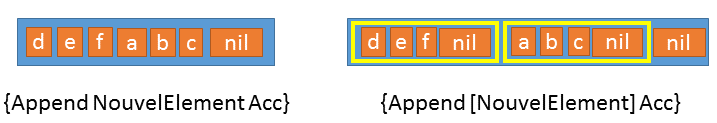
\includegraphics[width=10cm]{images/AstuceAppend.png}
	\caption{A gauche : une liste qu'il est impossible de reclasser dans le bon ordre. 
	A droite : une liste de listes qu'il est possible de reclasser dans le bon ordre en appelant Reverse.}
	\label{fig:astuceReverse}
\end{figure}

\section{Complexité calculatoire}
Comme nos fonctions peuvent Dans cette section, nous donnons les complexité calculatoire
propre de chaque fonction, c'est à dire sans tenir des sous-fonctions
utilisées.

	\begin{table}[ht!]
		\centering
			\begin{tabular}{|p{0.40\textwidth}|p{0.25\textwidth}|p{0.25\textwidth}|}
			\hline
			\textbf{Fonctions}																& \textbf{Temporelle}							& \textbf{Spatiale}	\\
			\hline
			InterpreteFlattened																& $n$ 														& $1$ \\
			\hline
			DureeTrans WantedDuration Part 										& $n$, taille de Part							& $1$ \\
			\hline 
			Etirer Facteur Part																& $n$, taille de Part 						& $1$ \\
			\hline
			Bourdon Note Part																	& $n$, taille de Part 						& $1$ \\
			\hline
			Transpose Demitons Part														& $n$, taille de Part 						& $1$ \\
			\hline
			Instrument InstrumentAtom Part										& $n$, taille de Part							& $1$ \\
			\hline
			VoiceDuration ListEchantillon											& $n$, taille de ListEchantillon	& $1$ \\
			\hline
			NumberOfSemiTones Note														& $1$ 														& $1$ \\
			\hline
			NameToNumber Name																	& $1$ 														& $1$ \\
			\hline
			ToNote Note																				& $1$ 														& $1$ \\ 
			\hline
			\hline
			MixMusic Music																		& $n$, taille de Music						& $1$ \\
			\hline
			MixVoice Voice																		& $n$, taille de Voice						& $1$ \\
			\hline
			Fill F Duree																			& $n$, valeur de Duree						& $1$ \\
			\hline
			Merge MusicsWithIntensity													& $n$, taille de MusicsWithIntensity	& $1$ \\
			\hline
			Combine L1 L2																			& $n$, taille de la plus grande des listes	& $1$ \\
			\hline
			Lissage AV Duree																	& $n$, taille de AV								& $1$ \\
			\hline
			HauteurToNote																			& $1$ 														& $1$ \\
			\hline
			NumberToNote																			& $1$ 														& $1$ \\
			\hline
			\end{tabular}
		\caption{Analyse de la complexité calculatoire de nos fonctions}
	\end{table}

\section{Extensions}
Nous avons créé deux extensions: la possibilité d'utiliser un instrument, d'une part, et une fonction de lissage de notes, d'autre part.

\subsection{Instrument}
Cette extension permet de mettre à profit le champ instrument: des échantillons. Pour ce faire, 
nous avons, comme suggéré dans les consignes, étendu la grammaire des transformations des 
partitions avec la transformation instrument(nom:). 
Ainsi, si le champ instrument: d'un échantillon n'est pas none, un fichier audio est chargé
et est répété aussi longtemps que désiré, grâce à notre sous-fonction \{RepetitionDuree Duree VecteurAudio\}. 

\subsection{Lissage}
Cette fonction permet de supprimer les bruits désagréables entre chaque note en adoucissant 
le début et la fin de ces dernières. Pour ce faire, nous avons modélisé une enveloppe sonore 
du type ADSR ("Attack - Decay - Sustain - Release")\footnote{Source: \url{http://fr.wikipedia.org/wiki/Enveloppe_sonore}}.
Cette enveloppe commence par une zone de croissance (Attack) jusqu'à un maximum, puis diminue (Decay) pour atteindre 
une zone stable (Sustain) et finalement la fin de la note (Release). Les différents paramètres de la courbe que 
nous avons introduits sont, pour une note d'une durée d'une seconde: 

\begin{itemize}
	\item Attack: durée de 0.1 s, passage d'une amplitude de 0 à 100\%;
	\item Decay: durée de 0.05 s, passage d'une amplitude de 100 à 90\%;
	\item Sustain: durée de 0.7 s;
	\item Release: durée de 0.15 s, passage d'une amplitude de 90 à 0\%.
\end{itemize}

Les paramètres de durée s'ajustent automatiquement en fonction de la durée de la note. 
Par ailleurs, chacun de ces paramètres peut être aisément modifié. 

Cette transformation est appliquée par défaut à tous les vecteurs audio synthétisés à partir d'un échantillon ou d'un instrument.

\begin{figure}[h!]
    \begin{minipage}[b]{0.4\linewidth}
        \centering 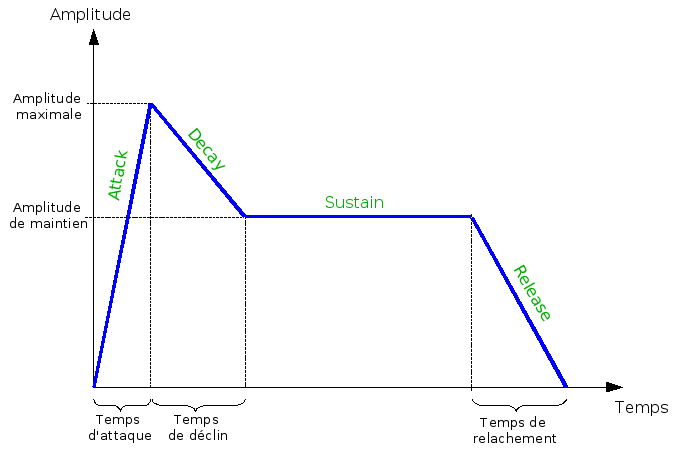
\includegraphics[height=6cm]{images/ADSR.png}
        \caption{Enveloppe sonore ADSR: modèle théorique}
    \end{minipage}\hfill
    \begin{minipage}[b]{0.48\linewidth}
        \centering 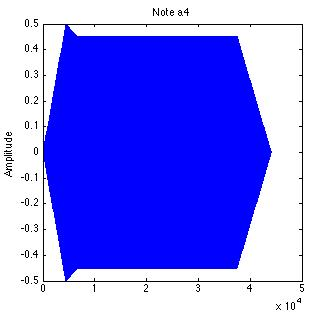
\includegraphics[height=6cm]{images/OurADSR.jpg}
        \caption{Affichage d'un de nos fichiers wave contenant une note lissée}
    \end{minipage}
\end{figure}

\section{Limitation du programme et difficultés perçues}
\subsection{Limitation du programme}
Le programme, bien qu'il fonctionne bien dans l'ensemble, pourrait être amélioré au niveau 
de la fonction Instrument. En effet, lorsque le fichier audio est trop court, ce dernier 
est simplement répété, ce qui peut laisser place à des effets assez étranges et non voulus,
puisque les fichiers audios à notre disposition simulent des instruments qui produisent
un son variable en fonction du temps. Une solution serait d'arriver à isoler une partie 
représentative des fichiers wav, et à ne reproduire que cette partie-là. Malheureusement, 
nous n'avons eu le temps que de réaliser de petites implémentations peut concluantes de 
cette méthode, et nous ne les avons pas présentées ici.
Par ailleurs, un autre amélioration de notre programme serait la gestion des erreurs, 
puisque il arrive très souvent qu'une partition ou une musique soit mal écrite dans le fichier .dj.oz.

\subsection{Difficultés rencontrées}
\subsubsection{Durée de compilation}
Le temps de compilation - parfois très long 
\newpage

% BROUILLONS

%\subsection{Fonction Interprete}
%\subsubsection{Sous-fonction principale}
%Cette fonction est codée autour de la sous-fonction fun {InterpreteFlattened FlattenedPartition},
 %qui parcourt la partition passée en paramètre et qui, à chaque itération, prend le premier
%élément de la liste, l'analyse (dans l'ordre: s'agit-il d'une transformation, d'un silence ou d'une note?)
 %et crée un échantillon. Cet échantillon est soit obtenu immédiatement s'il s'agit d'une note ou d'un
%silence (cas simple), soit après l'appel d'une autre sous-fonction s'il s'agit d'une transformation -
%chaque transformation ayant une fonction qui lui correspond (cas complexe). Par exemple, la sous-fonctioN
%{Etirer Facteur Part} est appelée pour la transformation etirer(facteur:F P). Ceci est vrai pour toutes
%les transformations, sauf muet(P), pour laquelle il n'existe pas de sous-fonction {Muet Part}.
%
%\subsubsection{Sous-fonctions de transformation}
%Comme dit ci-dessus, il y a autant de fonctions de transformation que de transformations (sauf pour muet(P)). 
%On retrouve donc :
%\begin{itemize}
	%\item \begin{verbatim} {WantedDuration Part} \end{verbatim}
	%\item \begin{verbatim} {Etirer Facteur Part} \end{verbatim}
	%\item \begin{verbatim} {Bourdon Note Part} \end{verbatim}
	%\item \begin{verbatim} {Transpose Demitons Part} \end{verbatim}
	%\item \begin{verbatim} {Instrument InstrumentAtom Part} \end{verbatim} 
%\end{itemize}
%
%Le fonctionnement  de chacune de ces sous-fonctions suit toujours le même schéma :
%\begin{itemize}
	%\item la partition passée en paramètre \verb Part  est transformée en une liste d'échantillon 
				%par un appel à \begin{verbatim} {InterpreteFlattend Partition} \end{verbatim} (la sous-fonction principale)
	%\item cette liste d'échantillons est ensuite parcourue par une sous-sous-fonction, qui applique 
				%la transformation demandée sur chacun des échantillons.
%\end{itemize} 
%
%Mettre un exemple?
%
%\subsubsection{Sous-fonctions complémentaires}
%Pour alléger certaines tâches de nos sous-fonctions de transformation,  nous avons créé 4 sous-fonctions complémentaires, à savoir:
%\begin{itemize}
	%\item {VoiceDuration ListEchantillon}
	%\item {NumberOfSemiTones Note}
	%\item {NameToNumber Name}
	%\item {ToNote Note}\footnote{Cette fonction nous a été donnée dans l'énonce du projet. Elle a été reprise sans être modifiée.}
%\end{itemize}
%
%La seule fonction qui présente ici un réel intérêt est la fonction {NumberOfSemiTones Note}. Nous l'expliquerons un peu plus loin.
%
%\subsection{Fonction Mix}
%\subsubsection{Sous-fonction principale}
%A l'instar de la fonction Interprete, Mix est codée autour d'une sous-fonction principale: 
%fun {MixMusic Music}, qui parcourt la musique (une liste de morceaux) passée en paramètre 
%et qui, à chaque itération, prend le premier élément de la liste, l'analyse d'après toutes
 %les possibilités que peut être un morceau et crée un vecteur audio. 
%De nouveau, deux cas se distinguent :
%\begin{itemize}
	%\item un cas simple: le vecteur audio peut être obtenu directement à partir d'une voix, 
				%d'une partition ou d'un vecteur audio déjà existant dans un fichier .wav.
	%\item un cas plus complexe, à savoir un filtre ou un merge (jouer deux musiques en même temps),
				%qui s'applique sur un vecteur audio déjà existant. Nous appelons ces cas 'complexes' car ils 
				%peuvent chacun s'appliquer sur un nouveau morceau, qui peut lui-même être soit simple soit complexe.
				%Il est en effet permis d'appliquer un filtre sur un filtre sur un filtre... A noter que l'extrémité 
				%d'une telle chaine est toujours un cas simple.
%\end{itemize}
%
%\subsubsection{Sous-fonctions de création de vecteur audio (cas simples)}
%Les 3 cas simples cités ci-dessus (voix, partition, wave)  ne nécessitent que l'utilisation
%de deux sous-fonctions (voix et partition reviennent au même, puisqu'il suffit d'appliquer Interprete sur partition()) :
%\begin{itemize}
	%\item {MixVoice Voice} (dont la méthode est donnée dans le rapport)
	%\item {Projet.readFile File} (fonction donnée)
%\end{itemize}
%
%\subsubsection{Sous-fonctions de filtre et merge (cas complexes)}
%Il y a autant de sous-fonction de filtre qu'il y a de filtres possibles (sauf pour renverser):
%\begin{itemize}
	%\item  {RepetitionNB NB AV}
	%\item {RepetitionDuree Duree AV}
	%\item {Clip Bas Haut AV}
	%\item ... (la suite de la liste se déduit assez facilement, et n'est pas particulièrement intéressante)
%\end{itemize}

\end{document}